\documentclass[conference]{IEEEtran}
\IEEEoverridecommandlockouts
\usepackage{cite}
\usepackage{amsmath,amssymb,amsfonts}
\usepackage{graphicx}
\usepackage{url}
\usepackage{textcomp}
\usepackage{booktabs}
\usepackage{tabularx}
\usepackage{flushend}
\usepackage{fancyhdr}
\setlength{\headheight}{17.15593pt}
\addtolength{\topmargin}{-5.15593pt}
\fancypagestyle{wieconfirst}{%
  \fancyhf{}%
  \fancyhead[L]{\footnotesize 2026 IEEE International Women in Engineering (WIE) Conference on Electrical and Computer Engineering (WIECON-ECE)\\30-31 October 2026, Southeast University, Dhaka, Bangladesh}%
  \fancyfoot[L]{\footnotesize 979-8-3195-1444-8/26/\$31.00~\copyright2026~IEEE}%
  \renewcommand{\headrulewidth}{0pt}%
  \renewcommand{\footrulewidth}{0pt}%
}

\begin{document}

\title{Leakage-Resistant Phishing URL Detection: Feature Engineering, Unsupervised Analysis, and Domain-Grouped Classifier Evaluation}

\author{%
\IEEEauthorblockN{Umme Habiba Moushi}%
\IEEEauthorblockA{\textit{Dept. of Computer Science}\\
\textit{and Engineering}\\
\textit{East West University}\\
A/2 Jahurul Islam Avenue, Aftabnagar\\
Dhaka 1212, Bangladesh\\
\texttt{2023-1-60-146@std.ewubd.edu}}%
\and%
\IEEEauthorblockN{Takia Labiba Razna}%
\IEEEauthorblockA{\textit{Dept. of Computer Science}\\
\textit{and Engineering}\\
\textit{East West University}\\
A/2 Jahurul Islam Avenue, Aftabnagar\\
Dhaka 1212, Bangladesh\\
\texttt{2023-1-60-170@std.ewubd.edu}}%
\and%
\IEEEauthorblockN{Ahmed Abdal Shafi Rasel}%
\IEEEauthorblockA{\textit{Dept. of Computer Science}\\
\textit{and Engineering}\\
\textit{East West University}\\
A/2 Jahurul Islam Avenue, Aftabnagar\\
Dhaka 1212, Bangladesh\\
\texttt{ahmed.shafi@ewubd.edu}}%
}

\maketitle
\thispagestyle{wieconfirst}
\pagestyle{empty}

\begin{abstract}
Phishing URLs lead users to fraudulent sites that steal credentials and other sensitive data. We evaluate six classifiers on URL-Phish, a dataset of 115{,}231 deduplicated URLs (98{,}641 benign and 16{,}590 phishing) described by 22 lexical and structural features plus the domain and top-level domain. Both the outer train/test split and the inner folds used for out-of-fold target encoding are grouped by domain. In a controlled comparison, row-wise inner folds cut phishing recall by 5 to 23 percentage points for five of the six models (most for Logistic Regression), even though the outer split held out whole domains. Among the six engineered-feature classifiers, the RBF-SVM did best on held-out domains: 96.92\% accuracy, 94.57\% phishing recall and 92.76\% precision, with a mean recall of $95.5\pm1.7\%$ over five repeated splits. Character $n$-gram models of the raw URL reached a higher phishing F1 (up to 97.17\%), but a domain split does not stop models from learning similarities between different domains. Applied unchanged to PhreshPhish, a dataset with different benign sources, the SVM's ROC-AUC fell from 0.993 to 0.762 and its false-positive rate rose from 2.3\% to 41.9\%. The training benign URLs are short, mostly HTTP landing pages, while the external benign URLs are long HTTPS deep links. Domain-grouped results on one dataset therefore do not show transfer to other data.
\end{abstract}

\begin{IEEEkeywords}
Phishing detection, machine learning, URL-Phish dataset, lexical features, domain-grouped evaluation, target encoding, Support Vector Machine, Random Forest, class imbalance
\end{IEEEkeywords}

\section{Introduction}
Phishing attacks imitate trusted services to steal credentials, financial data and other personal information. Blocklists react only after a site is reported, and content or visual detectors need access to the page, which adds latency. Lexical URL detection is fast and stateless because it uses only the URL string.

A row-wise split can put URLs from the same domain in both the training and test sets. Target encoding creates a related problem: even when the outer split holds out whole domains, row-wise inner folds let URLs from one domain inform one another's encodings. With such folds the training encoding carries domain-level label information, while an unseen test domain receives only the prior. We measure performance on new domains, with attention to missed phishing URLs, using domain-grouped splits at both levels on 115{,}231 URLs.

We first compare row-wise and domain-grouped inner folds with the features, encoder and models held fixed. We then evaluate six classifiers under domain grouping at both levels, using phishing-class metrics, domain-level bootstrap intervals, repeated splits and model selection on training data only, and compare them with gradient-boosted trees and raw-URL character $n$-grams on the same splits. Finally, we run feature ablations, compute how precision changes with the phishing base rate, and apply the trained pipelines to an external dataset to test whether the results transfer.

We do not propose a new method. The contribution is to quantify a specific failure mode of domain-grouped phishing benchmarks that use target encoding, and to show how far the resulting numbers transfer. Specifically: (i) row-wise inner encoding folds degrade recall on unseen domains even under a domain-grouped outer split; (ii) the RBF-SVM leads the engineered-feature models under phishing-class metrics, bootstrap intervals, repeated splits and training-only selection; (iii) raw-URL character $n$-grams and boosted trees are strong baselines under the same protocol; (iv) ablations and a base-rate analysis qualify the headline numbers; and (v) the performance does not transfer to a dataset with realistic benign URLs.

\section{Related Work}
Research on URL-based phishing detection covers lexical-feature models, systems that use page content, and character-level approaches.

\subsection{Prior Work on URL-Based Phishing Detection}
Several studies classify URLs with lexical features~\cite{gupta2021,butnaru2021}; others combine them with blocklists or visual similarity~\cite{rao2020}. Later work adds webpage or HTML features~\cite{asiri2023,aljofey2022} or uses ensembles and sequential models~\cite{karim2023,aslam2024}. URL-only filtering~\cite{alani2022} and character-level models~\cite{alshehri2022} are also relevant here. Benchmarking studies stress reproducible datasets and class balance~\cite{elaassal2020,hannousse2021}. Because these studies use different data and evaluation protocols, their accuracy figures are not comparable.

\subsection{Research Gap and Motivation}
Domain length, TLD, subdomain count and domain-substring entropy vary little among URLs from the same domain, so a row-wise split can let a model exploit domain identity instead of learning patterns that transfer to unseen domains. Group-aware validation is standard for clustered data~\cite{roberts2017}, and leakage is a known source of overly optimistic machine-learning results~\cite{kapoor2023}. A recent phishing benchmark found that many public datasets lack standard test splits or use random ones, and it addresses leakage with temporal evaluation and similarity-based pruning~\cite{dalton2025}. The same study shows that precision must be read against the phishing base rate~\cite{dalton2025}. We examine a different source of leakage: row-wise inner folds can make target-encoded domain values informative during training even when the outer split holds out domains. We also include character-level URL models~\cite{alshehri2022}, which need no manual feature extraction.

\section{Dataset Description}

\subsection{URL-Phish Dataset Overview}
URL-Phish~\cite{linh2026} has 116{,}600 records: 100{,}000 benign URLs from ROR~\cite{ror2025}, educational and governmental domains, and ranked sites, and 16{,}600 phishing URLs from PhishTank~\cite{phishtank} collected between November 2024 and September 2025. After removing 1{,}369 duplicate rows, 115{,}231 URLs remain (98{,}641 benign and 16{,}590 phishing; an imbalance of 5.95:1).

The CSV has 26 columns: 22 numeric features, \texttt{url}, \texttt{dom}, \texttt{tld} and the binary label. The engineered-feature models drop \texttt{url} and target-encode \texttt{dom} and \texttt{tld}. Here \texttt{dom} is the registrable domain and \texttt{tld} the public suffix. A \texttt{tldextract} check found two \texttt{dom} values (\texttt{cgs.gov.cz}, \texttt{szpi.gov.cz}) that are not registrable domains, and no \texttt{dom} value, or registrable domain derived from it, is shared between the training and test sets.

\subsection{Domain-Grouped Train/Test Split}
We split with \texttt{GroupShuffleSplit} on \texttt{dom} (80/20 target, seed 42). Because domains differ in size, the split gave 89{,}251 training URLs (77.4\%; 78{,}905 benign, 10{,}346 phishing) and 25{,}980 test URLs (22.6\%; 19{,}736 benign, 6{,}244 phishing), with no domain overlap. Phishing prevalence is 11.6\% in training and 24.0\% in test (14.4\% overall), so accuracy is not comparable with a balanced setting.

\section{Feature Engineering and Descriptive Analysis}
We extracted 22 numeric URL features: \texttt{url\_len}, \texttt{dom\_len}, \texttt{is\_ip}, \texttt{tld\_len}, \texttt{subdom\_cnt}, character and punctuation counts, character ratios, \texttt{is\_https}, \texttt{slash\_cnt}, \texttt{entropy}, \texttt{path\_len} and \texttt{query\_len}. The models also use target-encoded \texttt{dom} and \texttt{tld}; the raw URL is excluded. No feature pair was collinear enough to justify removal. Digit ratio ($r=0.518$), entropy ($r=0.513$), HTTPS usage ($r=0.400$), digit count ($r=0.329$) and URL length ($r=0.324$) correlate most strongly with the label; these are univariate associations, not causal or model-specific importances.

Phishing URLs were longer on average than benign ones (56.31 vs.\ 29.10 characters), had higher entropy (4.32 vs.\ 3.79) and longer paths (17.16 vs.\ 4.62 characters). HTTPS appeared in 91.4\% of phishing URLs and 34.9\% of benign URLs. These contrasts may partly reflect the sources: benign URLs came from institutional and ranked-site lists and often had short or missing paths.

\section{Methodology}
\label{sec:methodology}

\subsection{Data Cleaning and Leakage-Resistant Preprocessing}
All model-facing preprocessing was fitted on training data, and every classifier used the same feature pipeline. Fourteen missing \texttt{tld} values were filled with the global mode before splitting (the same value the training partition yields), and exact duplicates were removed before splitting. We target-encoded \texttt{dom} and \texttt{tld} with the smoothed out-of-fold scheme of Micci-Barreca~\cite{micci2001}, using smoothing 10 and five inner folds grouped by domain, so no training URL was encoded with labels from its own domain. Unseen test domains map to the training prior for \texttt{dom}, while \texttt{tld} can still vary. Numeric features were standardized on the training data, and estimators that support it used balanced class weights. All steps were fitted inside the training pipeline.

\subsection{Classifier Training and Configuration}
We evaluated Logistic Regression (at most 1{,}000 iterations), a Decision Tree (depth 6, minimum leaf size 10), Gaussian Naive Bayes (defaults), a Random Forest (200 trees, depth 8, minimum split 20, minimum leaf 10), a Stacking ensemble and an RBF-SVM ($C=1$). Stacking combines Logistic Regression ($C=0.1$), a depth-6 tree with minimum leaf size 10 and a 100-tree forest with depth 8 and minimum leaf 10, with a Logistic Regression meta-learner. The trees, forests and SVM used balanced class weights; Logistic Regression and Naive Bayes kept the default class settings. Each model has its own pipeline and all share the same split and preprocessing, so differences come mainly from the learning algorithms.

\subsection{Unsupervised Analysis of the Feature Space}
We standardized the 22 numeric features and ran K-Means for $k=2$ to 9. Inertia showed no clear elbow, so $k=2$ is only an exploratory, task-motivated choice. It gave a silhouette score of 0.754 and a moderate association with the labels ($\chi^2=9599.75$, $p<0.001$, Cram\'er's $V\approx0.29$, computed as $\sqrt{\chi^2/n}$ for a $2\times2$ table; with 115{,}231 observations the test is significant by sample size alone, so the effect size matters more). The smaller cluster has 2{,}248 URLs, 86.3\% of them phishing, but holds only 1{,}939 of the 16{,}590 phishing URLs (11.7\%); the larger cluster has 14{,}651 phishing and 98{,}332 benign URLs. The high silhouette score therefore reflects a compact minority group, not a benign/phishing partition. The clusters were not classifier inputs. The analysis shows that the feature structure alone does not separate the classes, which is why the supervised protocol matters.

\subsection{Evaluation Framework}
The domain-held-out test set has 25{,}980 URLs (24.0\% phishing). We report accuracy, weighted F1, phishing precision, recall and F1, balanced accuracy and MCC. Intervals are 95\% bootstrap intervals that resample whole test domains (1{,}000 draws), plus mean\,$\pm$\,SD over five further grouped splits (seeds 0 to 4). Models were selected by grouped five-fold cross-validation on the training set; the test set was used only for the final comparison, and hyperparameters were fixed in advance. Phishing recall was the primary selection metric and balanced accuracy the secondary one. Four baselines used the same splits, and Section~\ref{sec:external} describes an external test of the fixed pipelines.

\section{Experimental Results and Analysis}
\label{sec:results}

\subsection{Overall Performance Comparison}
Table~\ref{tab:performance} gives overall and phishing-class metrics on the domain-held-out test set. Among the six classifiers, the RBF-SVM has the highest accuracy (96.92\%), phishing recall (94.57\%), phishing F1 (93.66\%), balanced accuracy (96.12\%) and MCC (0.916). Logistic Regression and Stacking have higher phishing precision (96.70\% and 96.33\%) but miss many more phishing URLs (recall 79.21\% and 80.62\%). Naive Bayes is worst, which fits its conditional-independence assumption being a poor match for correlated lexical counts. Weighted recall equals accuracy and is omitted.

\begin{table}[htbp]
\centering
\caption{Overall and Phishing-Class Metrics on the Domain-Held-Out Test Set (\%; Test Set 76\% Benign)}
\label{tab:performance}
\small
\resizebox{\linewidth}{!}{%
\begin{tabular}{lrrrrrrr}
\toprule
Model & Acc. & Wtd F1 & Prec. & Recall & F1 & Bal.\ Acc. & MCC \\
\midrule
SVM (RBF) & 96.92 & 96.93 & 92.76 & 94.57 & 93.66 & 96.12 & 0.916 \\
Random Forest & 94.73 & 94.72 & 89.46 & 88.52 & 88.99 & 92.61 & 0.855 \\
Stacking & 94.60 & 94.43 & 96.33 & 80.62 & 87.78 & 89.82 & 0.849 \\
Logistic Regression & 94.35 & 94.15 & 96.70 & 79.21 & 87.09 & 89.18 & 0.842 \\
Decision Tree & 93.01 & 92.99 & 85.94 & 84.77 & 85.35 & 90.19 & 0.808 \\
Naive Bayes & 85.14 & 83.99 & 79.04 & 51.95 & 62.70 & 73.80 & 0.558 \\
\bottomrule
\end{tabular}
}
\end{table}

\subsection{Confusion Matrix Analysis}
Table~\ref{tab:confusion} gives counts and domain-bootstrap intervals for the 6{,}244 phishing and 19{,}736 benign test URLs, and Fig.~\ref{fig:cms} shows the matrices. The RBF-SVM has the fewest false negatives (339); Logistic Regression and Stacking have the fewest false positives (169 and 192). The SVM recall interval (0.935 to 0.965) is narrower than those for Random Forest (0.802 to 0.985) and Stacking (0.696 to 0.939), so the recall of those models depends more on which domains are held out.

\begin{table}[htbp]
\centering
\caption{Confusion Matrix Breakdown and Phishing-Recall 95\% Domain-Bootstrap Interval}
\label{tab:confusion}
\small
\resizebox{\linewidth}{!}{%
\begin{tabular}{lrrrrc}
\toprule
Model & TP & TN & FP & FN & Recall 95\% CI \\
\midrule
SVM (RBF) & 5,905 & 19,275 & 461 & 339 & 0.935 to 0.965 \\
Random Forest & 5,527 & 19,085 & 651 & 717 & 0.802 to 0.985 \\
Stacking & 5,034 & 19,544 & 192 & 1,210 & 0.696 to 0.939 \\
Logistic Regression & 4,946 & 19,567 & 169 & 1,298 & 0.710 to 0.890 \\
Decision Tree & 5,293 & 18,870 & 866 & 951 & 0.756 to 0.957 \\
Naive Bayes & 3,244 & 18,876 & 860 & 3,000 & 0.254 to 0.841 \\
\bottomrule
\end{tabular}
}
\end{table}

\begin{figure}[t]
\centering
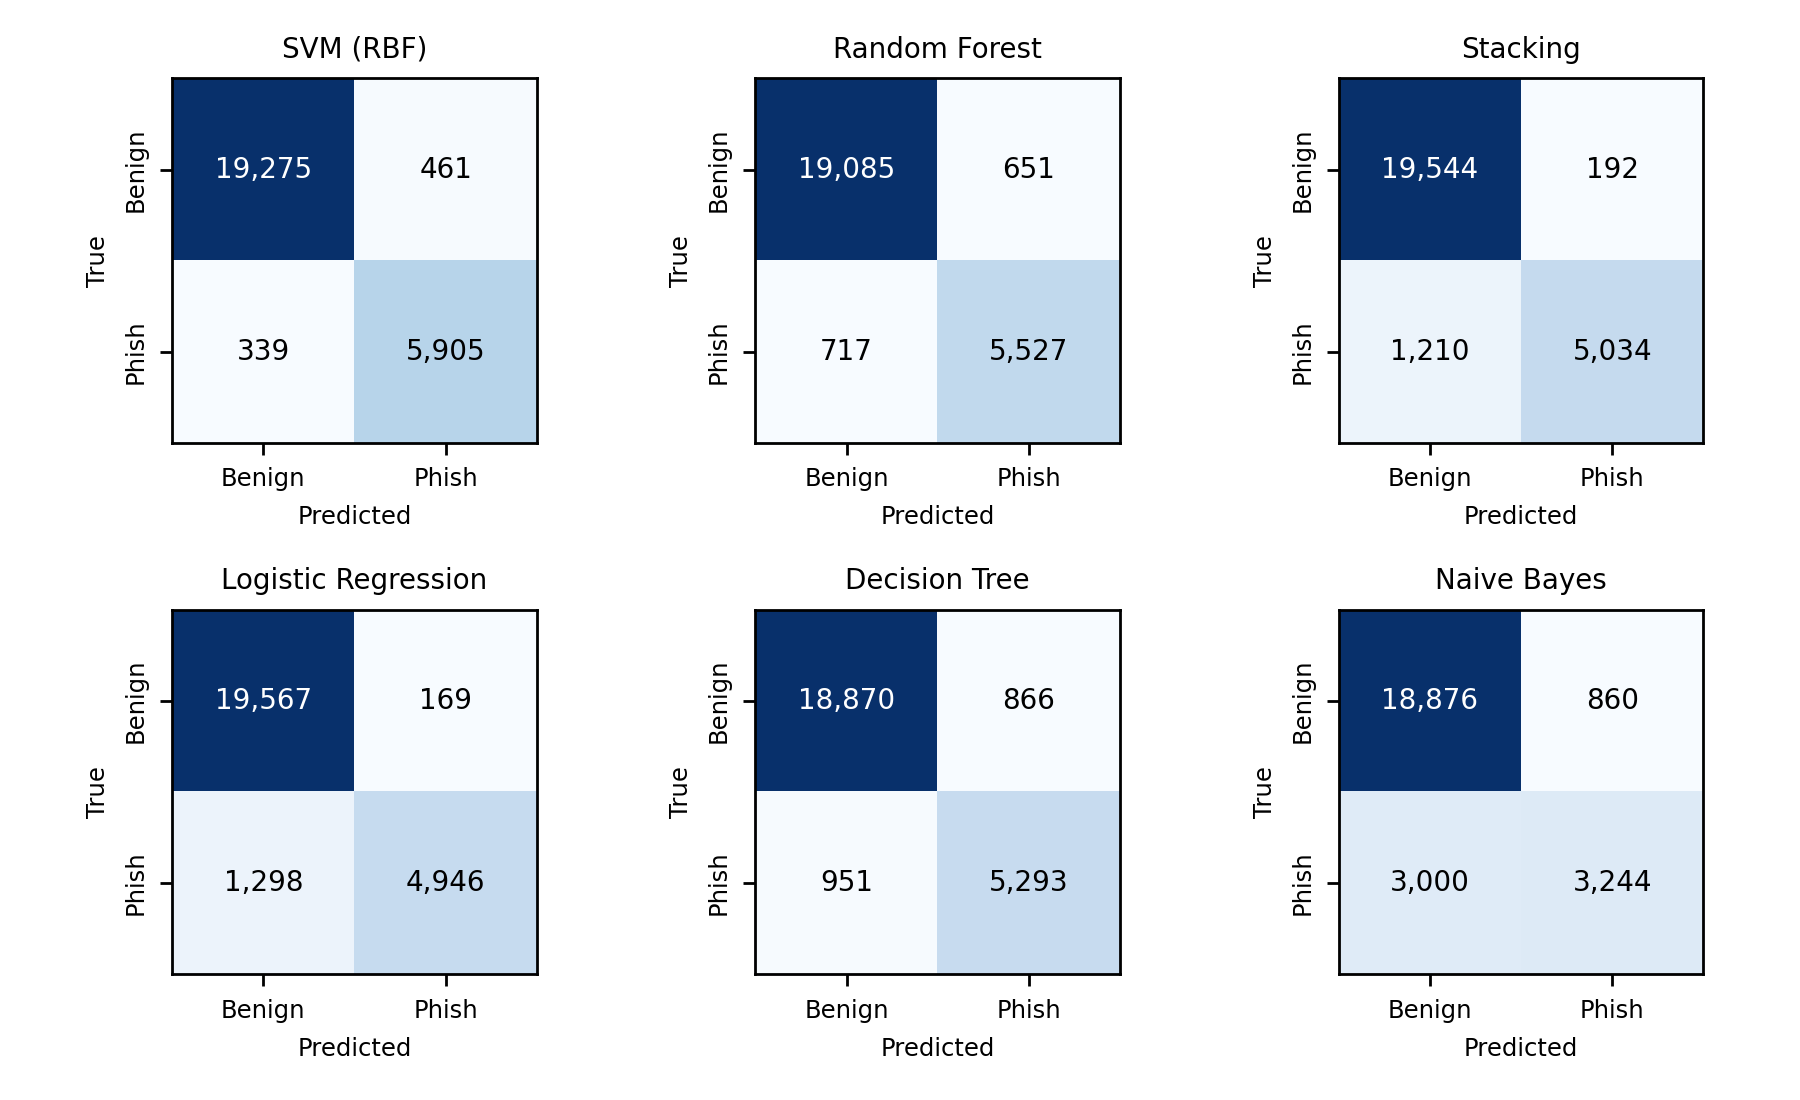
\includegraphics[width=0.72\linewidth]{fig_cm_grid.png}
\caption{Confusion matrices for the six classifiers on the domain-held-out test set.}
\label{fig:cms}
\end{figure}

\subsection{Model Selection on Training Data}
\label{sec:selection}
Grouped five-fold cross-validation selected the SVM under the recall-first criterion, narrowly: recall 0.945 and balanced accuracy 0.961, against 0.942 recall for Random Forest. Stacking had the highest F1 ($0.904\pm0.028$; SVM $0.888\pm0.022$) but scored lower on the held-out set (F1 87.78\% vs.\ 93.66\%; recall 80.62\% vs.\ 94.57\%).

\subsection{Repeated Domain-Grouped Splits}
Over five grouped splits the SVM had the highest mean F1 (0.911) and recall (0.955, SD 0.017). Its F1 was above that of Logistic Regression, Decision Tree, Naive Bayes and Random Forest in all five splits, and above Stacking's in three. With five pairs the smallest attainable two-sided Wilcoxon $p$ is 0.0625, so these comparisons cannot establish significance. The seed-42 headline split favored the SVM (F1 0.937 vs.\ a repeated-split mean of 0.911).

\begin{table}[htbp]
\centering
\caption{Mean $\pm$ SD over Five Repeated Domain-Grouped Splits}
\label{tab:repeated}
\small
\resizebox{\linewidth}{!}{%
\begin{tabular}{lccccc}
\toprule
Model & Acc. & Prec. & Recall & F1 & Bal.\ Acc. \\
\midrule
SVM (RBF) & .972$\pm$.003 & .872$\pm$.052 & .955$\pm$.017 & .911$\pm$.033 & .965$\pm$.008 \\
Stacking & .964$\pm$.019 & .930$\pm$.032 & .846$\pm$.069 & .885$\pm$.038 & .918$\pm$.035 \\
Random Forest & .957$\pm$.012 & .835$\pm$.070 & .905$\pm$.060 & .866$\pm$.041 & .937$\pm$.029 \\
Logistic Regression & .960$\pm$.012 & .920$\pm$.038 & .814$\pm$.052 & .863$\pm$.040 & .901$\pm$.026 \\
Decision Tree & .940$\pm$.020 & .762$\pm$.113 & .886$\pm$.120 & .811$\pm$.086 & .919$\pm$.057 \\
Naive Bayes & .893$\pm$.040 & .696$\pm$.119 & .571$\pm$.165 & .619$\pm$.128 & .764$\pm$.082 \\
\bottomrule
\end{tabular}
}
\end{table}

\subsection{Split, Encoding and Domain Leakage}
\label{sec:comparison}
Table~\ref{tab:controlled} holds features, encoder and model settings fixed and changes only the folds. A uses row-wise outer and inner folds; B groups the outer split but not the inner folds; C groups both by domain.

From B to C, recall rose for five of six models: Logistic Regression (0.562 to 0.792), Decision Tree (0.649 to 0.848), Random Forest (0.751 to 0.885), Stacking (0.670 to 0.806) and SVM (0.897 to 0.946); Naive Bayes was essentially unchanged (0.505 to 0.520). In the training data of B, the row-wise out-of-fold encoding of \texttt{dom} correlated 0.74 with the label, although every test domain was unseen and mapped to the prior. Balanced accuracies follow the same pattern (SVM: .978 in A, .940 in B and .961 in C; Logistic Regression: .953, .780 and .892).

A and C also differ in domain overlap and prevalence, so their gap is not a pure estimate of domain leakage. In A, only 23.8\% of test URLs shared a domain with training, and prevalence was 14.4\% in A against 24.0\% in C. The accuracy changes therefore mix domain novelty, class prevalence and the concentration of phishing URLs in a few domains.

\begin{table}[htbp]
\centering
\caption{Controlled Comparison: Accuracy / Phishing Recall}
\label{tab:controlled}
\small
\resizebox{\linewidth}{!}{%
\begin{tabular}{lccc}
\toprule
Model & A: row split, row inner & B: domain split, row inner & C: domain split, grouped inner \\
\midrule
SVM (RBF) & .984 / .969 & .962 / .897 & .969 / .946 \\
Random Forest & .986 / .964 & .927 / .751 & .947 / .885 \\
Stacking & .990 / .955 & .915 / .670 & .946 / .806 \\
Logistic Regression & .984 / .910 & .893 / .562 & .944 / .792 \\
Decision Tree & .981 / .948 & .899 / .649 & .930 / .848 \\
Naive Bayes & .942 / .845 & .852 / .505 & .851 / .520 \\
\bottomrule
\end{tabular}
}
\end{table}

\subsection{Feature Ablations}
Removing \texttt{dom} changed F1 by at most 0.002; removing \texttt{dom} and \texttt{tld} together lowered SVM F1 from 0.937 to 0.922. Removing HTTPS lowered F1 for every model (by 0.014 for the SVM and 0.074 for the Decision Tree). Removing path and query features hurt Logistic Regression most (0.871 to 0.763); the SVM was least affected among the models that lost F1 (0.937 to 0.927), while the Decision Tree and Naive Bayes were unchanged or slightly better.

\begin{table}[htbp]
\centering
\caption{Phishing F1 under Feature Ablations (Headline Split)}
\label{tab:ablation}
\small
\resizebox{\linewidth}{!}{%
\begin{tabular}{lccccc}
\toprule
Model & Full & No \texttt{dom} & No \texttt{dom}, \texttt{tld} & No path/query & No HTTPS \\
\midrule
SVM (RBF) & .937 & .937 & .922 & .927 & .923 \\
Random Forest & .890 & .892 & .882 & .889 & .860 \\
Stacking & .878 & .877 & .871 & .860 & .854 \\
Logistic Regression & .871 & .871 & .861 & .763 & .853 \\
Decision Tree & .854 & .854 & .847 & .858 & .780 \\
Naive Bayes & .627 & .627 & .577 & .664 & .622 \\
\bottomrule
\end{tabular}
}
\end{table}

\subsection{Comparison with Representative Baselines}
\label{sec:baselines}
On the same grouped splits we trained gradient-boosted trees on the engineered features and TF-IDF character 3-to-5-gram models on the raw URL. XGBoost~\cite{chen2016xgboost} used 300 trees of depth 6 with learning rate 0.1 and class-weight scaling; HistGradientBoosting used balanced class weights; the $n$-gram models used at most 300{,}000 features with minimum document frequency 2 and sublinear term-frequency weighting, a Logistic Regression (at most 2{,}000 iterations) or linear SVM classifier, balanced class weights and otherwise default settings. Table~\ref{tab:baselines} gives the results.

XGBoost and HistGradientBoosting come close to the RBF-SVM on phishing F1 (93.38\% and 92.78\% vs.\ 93.66\%). On the headline split, the character $n$-gram SVM reaches 97.17\% F1 and its Logistic Regression counterpart has the highest recall (98.75\%). Over repeated splits their mean F1 is 0.948 and 0.946, against 0.911 for the RBF-SVM, but the $n$-gram SVM's mean recall is lower (0.911 vs.\ 0.955).

A domain split tests new domains, but it does not separate URLs that share a template, hosting service or campaign string across different domains. Character $n$-grams can learn those similarities, and also differences in how benign and phishing URLs were collected, such as their schemes and host strings. We read the higher scores as evidence that the engineered features leave information unused on this dataset, not as evidence that $n$-gram models generalize better to new campaigns. Testing that needs a temporal or similarity-based evaluation.

\begin{table}[htbp]
\centering
\caption{Baselines under the Same Domain-Grouped Protocol. Left: Headline Split (\%). Right: Mean $\pm$ SD over Five Repeated Splits}
\label{tab:baselines}
\small
\resizebox{\linewidth}{!}{%
\begin{tabular}{lrrrrrrcc}
\toprule
Model & Acc. & Prec. & Rec. & F1 & Bal.\ Acc. & MCC & F1 (5 splits) & Rec. (5 splits) \\
\midrule
Char $n$-gram SVM & 98.66 & 99.08 & 95.32 & 97.17 & 97.52 & 0.963 & .948$\pm$.025 & .911$\pm$.045 \\
Char $n$-gram LR & 98.09 & 93.65 & 98.75 & 96.13 & 98.32 & 0.949 & .946$\pm$.033 & .954$\pm$.038 \\
XGBoost & 96.84 & 93.98 & 92.78 & 93.38 & 95.45 & 0.913 & .911$\pm$.031 & .931$\pm$.035 \\
HistGradientBoosting & 96.56 & 93.52 & 92.04 & 92.78 & 95.01 & 0.905 & .912$\pm$.033 & .937$\pm$.031 \\
RBF-SVM (Table~\ref{tab:performance}) & 96.92 & 92.76 & 94.57 & 93.66 & 96.12 & 0.916 & .911$\pm$.033 & .955$\pm$.017 \\
\bottomrule
\end{tabular}
}
\end{table}

\subsection{Cross-Dataset Evaluation on PhreshPhish}
\label{sec:external}
To test transfer, we applied the six pipelines trained on the URL-Phish training split, with no retraining and no threshold changes, to the test file of PhreshPhish~\cite{dalton2025}, which contains benign and phishing pages collected from the web. After removing duplicates and 288 URLs that also occur in URL-Phish (normalized match), 166{,}268 URLs remained, and we drew a random sample of 30{,}000 (45.7\% phishing). We recomputed the 22 features from the URL string with an extractor that reproduced every URL-Phish feature column on a 6{,}000-URL sample, and derived \texttt{dom} and \texttt{tld} with \texttt{tldextract}. Recall and false-positive rate do not depend on the external prevalence, so Table~\ref{tab:external} compares those.

Every model degraded sharply. The SVM's recall fell from 0.946 to 0.790, its false-positive rate rose from 0.023 to 0.419 and its ROC-AUC fell from 0.993 to 0.762; the other models' false-positive rates were 0.29 to 0.69. On the 24{,}269 URLs whose domain was not in the training split, the SVM had recall 0.748, a false-positive rate of 0.448 and AUC 0.705. At the measured external recall and false-positive rate, the SVM's precision would be 9.0\% at a 5\% phishing base rate and 1.9\% at 1\%.

The feature distributions explain the drop. In URL-Phish, benign URLs average 29.1 characters, with a mean path length of 4.6 and 34.9\% HTTPS, so the benign class is mostly short landing pages. In the PhreshPhish sample, benign URLs average 59.2 characters, with a mean path length of 33.9 and 97.8\% HTTPS (phishing URLs: 63.9, 15.6 and 85.4\%); they are long HTTPS deep links such as news articles. The URL-Phish models learned that long paths and HTTPS indicate phishing, so they flagged 41.9\% of the external benign URLs (SVM). Setting \texttt{is\_https} to its training mean lowered the SVM's false-positive rate to 0.236 but also its recall to 0.710. Part of the separability within URL-Phish therefore reflects its benign sources and the HTTPS and path-length contrasts. We did not evaluate the $n$-gram and boosted-tree baselines externally, so we make no claim about their transfer.

\begin{table}[htbp]
\centering
\caption{Fixed URL-Phish-Trained Pipelines: URL-Phish Test Set vs.\ PhreshPhish Sample (No Retraining)}
\label{tab:external}
\small
\resizebox{\linewidth}{!}{%
\begin{tabular}{lcccccc}
\toprule
 & \multicolumn{3}{c}{URL-Phish test} & \multicolumn{3}{c}{PhreshPhish sample} \\
\cmidrule(lr){2-4}\cmidrule(lr){5-7}
Model & Recall & FPR & AUC & Recall & FPR & AUC \\
\midrule
SVM (RBF) & .946 & .023 & .993 & .790 & .419 & .762 \\
Random Forest & .885 & .033 & .988 & .833 & .694 & .635 \\
Stacking & .806 & .010 & .989 & .723 & .459 & .672 \\
Logistic Regression & .792 & .009 & .988 & .669 & .294 & .749 \\
Decision Tree & .848 & .044 & .979 & .818 & .670 & .655 \\
Naive Bayes & .520 & .044 & .934 & .537 & .463 & .479 \\
\bottomrule
\end{tabular}
}
\end{table}

\section{Discussion and Limitations}

\subsection{Deployment and Base Rates}
URL-only inputs allow screening before the page is fetched. On the URL-Phish test set the RBF-SVM missed 339 of 6{,}244 phishing URLs and had 92.8\% precision, but these figures do not carry over: on the PhreshPhish sample its false-positive rate was 41.9\%. Table~\ref{tab:baserate} recalculates precision at lower base rates from the measured recall and false-positive rates. These estimates are optimistic because the benign URLs come from institutional and ranked-site sources. We would use such a model only after retraining and validating it on benign traffic with realistic deep links.

\begin{table}[htbp]
\centering
\caption{Precision (\%) Implied by Measured Recall and False-Positive Rate at Different Base Rates}
\label{tab:baserate}
\small
\begin{tabular}{lrrrrr}
\toprule
Model & Recall & FPR & 14.4\% & 5\% & 1\% \\
\midrule
SVM (RBF) & 94.6 & 2.3 & 87.2 & 68.1 & 29.0 \\
Random Forest & 88.5 & 3.3 & 81.9 & 58.5 & 21.3 \\
Stacking & 80.6 & 1.0 & 93.3 & 81.3 & 45.6 \\
Logistic Regression & 79.2 & 0.9 & 94.0 & 83.0 & 48.3 \\
Decision Tree & 84.8 & 4.4 & 76.5 & 50.4 & 16.3 \\
Naive Bayes & 52.0 & 4.4 & 66.7 & 38.6 & 10.7 \\
\midrule
XGBoost & 92.8 & 1.9 & 89.3 & 72.2 & 33.3 \\
Char $n$-gram SVM & 95.3 & 0.3 & 98.3 & 94.7 & 77.6 \\
Char $n$-gram LR & 98.8 & 2.1 & 88.7 & 71.0 & 32.0 \\
\bottomrule
\end{tabular}
\end{table}

\subsection{Limitations}
\label{sec:limitations}
The data cover November 2024 to September 2025 and may not reflect later phishing patterns. Because the models use only URL structure and text, they can miss phishing pages on compromised legitimate domains and can be evaded by URLs built to look benign.

The benign URLs come from institutional and ranked-site sources, with a mean path length of 4.6 characters against 17.2 for phishing URLs, which suggests many are landing pages. Every URL carries an explicit scheme, so the HTTPS gap (34.9\% benign, 91.4\% phishing) reflects the links the benign sources serve, not missing scheme information. The ablations show the models use this signal, and the cross-dataset test shows it matters: URL-Phish models flagged 41.9\% (SVM) to 69.4\% (Random Forest) of the benign URLs of an external dataset.

The test set has a higher phishing prevalence than the training set (24.0\% vs.\ 11.6\%), which affects accuracy and precision. Phishing URLs are concentrated in fewer domains, so results vary with the split: across repeated splits, recall SDs are 0.05 to 0.16 for every model except the SVM. Only five repeated splits were run, so they say little about statistical differences. We used one training dataset and one hyperparameter configuration per model. The external test covers one dataset, a 30{,}000-URL sample and only the six feature-based pipelines. We do not compare with published detectors because their datasets and protocols differ.

We group by the supplied \texttt{dom} value, the registrable domain, and do not merge domains that differ only by subdomain or registrar-level variation. Stacking's internal cross-validation is row-wise, which may affect its meta-learner weights. Grouping by domain also leaves cross-domain similarity untouched, so character $n$-gram models may be especially sensitive to shared templates, hosts or phishing kits, and the baselines use default settings. Temporal and similarity-based splits for all approaches remain future work.

\subsection{Interpreting the Results}
With row-wise inner folds, URLs from one domain help determine one another's target-encoded values, even though a held-out domain has no such label history and receives the training prior. Grouping the inner folds removes that mismatch. The recall gains from B to C in Table~\ref{tab:controlled} fit this explanation, but they are not a precise causal estimate because the splits also differ in prevalence and in which domains are held out. Removing \texttt{dom} changed phishing F1 by at most 0.002, so explicit domain encoding added little on this split.

The SVM favors recall and catches 5{,}905 of 6{,}244 phishing URLs, while Logistic Regression and Stacking make fewer false-positive errors but miss more. URLs from one domain are not independent, so resampling whole test domains describes variability better than resampling rows; the SVM's recall interval (0.935 to 0.965) is much narrower than those of Random Forest and Stacking. The character $n$-gram SVM's higher F1 does not make it uniformly better: its mean recall over repeated splits was below the feature-based SVM's.

The evidence supports a narrower claim than ``the best phishing detector'': domain-grouped target encoding avoids a training and deployment mismatch, and the RBF-SVM is a strong recall-oriented option on URL-Phish. The cross-dataset result shows that this performance is specific to the dataset's benign sources. A stronger assessment would keep domains separated, add time-based and similarity-based holdouts, train and test on benign traffic with realistic deep links, and choose a threshold from the relative costs of missed phishing and false alarms.

\section{Conclusion and Future Work}
Grouping the outer split by domain is not enough if the target-encoding folds stay row-wise: phishing recall fell by 5 to 23 percentage points for five of the six models (most for Logistic Regression). With domain-grouped folds at both levels, the RBF-SVM led the six feature-based classifiers on the held-out domains of URL-Phish, with 96.92\% accuracy, 94.57\% recall and 92.76\% precision and a mean recall of $95.5\pm1.7\%$ over five repeated splits. Its F1 advantage over Stacking was not statistically distinguishable, and boosted trees performed comparably. Raw-URL character $n$-grams scored a higher F1, but grouping by domain does not control for similarity between different domains, so their scores do not show better performance on new campaigns.

The main limitation is transfer. Applied unchanged to PhreshPhish, every pipeline degraded sharply (SVM ROC-AUC 0.993 to 0.762, false-positive rate 2.3\% to 41.9\%), because URL-Phish's benign URLs are short, mostly HTTP landing pages while realistic benign URLs are long HTTPS deep links. Precision also falls as the phishing base rate drops, and the HTTPS signal partly reflects dataset provenance. Domain-grouped evaluation on one dataset is therefore necessary but not sufficient. Future work should train on data with realistic benign deep links, test temporal and similarity-based splits, evaluate the character-level and boosted-tree models externally, and try hybrid lexical and content models.

\section*{Reproducibility and Data Availability}
The headline split uses \texttt{random\_state=42} and the repeated splits use seeds 0 to 4. The experiments use scikit-learn~\cite{pedregosa2011}.
The URL-Phish dataset analyzed in this study is publicly available on Mendeley Data~\cite{linh2026} (\url{https://data.mendeley.com/datasets/65z9twcx3r/2}).
The PhreshPhish benchmark used for cross-dataset evaluation is publicly available~\cite{dalton2025} (arXiv:2507.10854).
Code that generates all tables and figures, with the saved outputs of the runs reported here, is at \url{https://github.com/UmmeHabibaMoushi/leakage-resistant-phishing-url-detection}.

\section*{Acknowledgment}
Generative AI (Claude, Anthropic) was used to assist with analysis code, drafting and editing text, and LaTeX formatting. The authors designed the study, ran all experiments, checked the reported numbers against the outputs, and take full responsibility for the content.

\bibliographystyle{IEEEtran}
\bibliography{Phisingbib}

\end{document}
